\chapter{Data}

Fetal therapy is a promising field in pediatric medicine, and prenatal surgery has become an option for an increasing number of babies with congenital disabilities. Regardless of its popularity increase, it is still a relatively rare procedure as it affects only a small percentage of pregnancies and offers risks for both the mother and the unborn baby. The procedure is also highly sophisticated and thus requires a skilled team, assisted with advanced technological resources to perform such complex procedures. The particularities of this topic, make research in the field very challenging.

At the same time, as fetuses are protected against biological and social effects while in utero, the circumstances offer an excellent opportunity for investigation of fetal behavior free of influences from the outside world. The study of fetal pain is a great example, as it is still a topic of debate if human fetuses feel pain or not. The Fetal Pain Study Group from the University of São Paulo was formed with the purpose of helping answer these questions. In the following section, we describe one of their most recent studies, which consisted of the assessment of pain trough facial expressions in fetuses.

\section{Fetal Pain Study}

Trough the use of high definition 4-D ultrasound machines, it is possible to record and observe fetal responses to different stimuli, and by looking at their facial expressions and body movements, one could potentially assess visual pain responses during the intrauterine life. This was done by the aforementioned study group, which proved the feasibility of using a pain scale, initially developed for acute pain assessment in neonates, in fetuses \citep{bernardes2018feasibility}. 

Based on this hypothesis, the Fetal Pain Study Group conducted a novel study, which is the first attempt to assess specific pain-related facial patterns in human fetuses. They were able to evaluate facial expressions after an anesthetic injection was administered before an intrauterine surgical procedure, which was used as a model of acute pain. They were pioneer in the usage of two ultrasound machines for this purpose, as the exact moment of the anesthetic puncture was recorded to capture the reaction of the fetus and its manifestations of pain. 

While one machine was used to perform the anesthesia, a second ultrasound machine was placed in the clinical room and operated by a fetal medicine specialist to monitor the fetus’s face and its expressions. The spatial set-up of the room can be seen in Figure \ref{fig:ultrasound}.

\begin{figure}[h!tp]
    \centering
    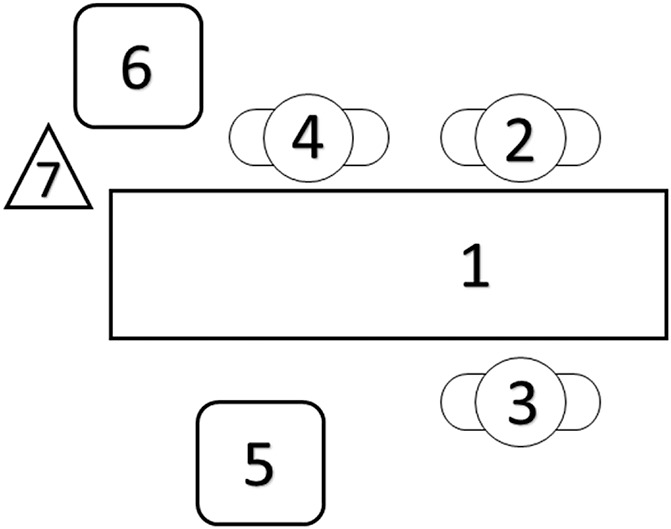
\includegraphics[width=.35\textwidth]{imgs/chap4_ultrasound_setup.jpg}
    \caption[Operating room set-up for surgery and face recording]{Operating room set-up for surgery and face recording. (1) Position of the mother; (2) chief surgeon who performed the puncture; (3) assistant surgeon who obtained the 4-D images; (4) surgical technologist; (5) ultrasound machine used in surgery focusing the fetal trachea/thigh; (6) ultrasound machine used for fetal face recording; and (7) an external camera. Diagram extracted from \citep{bernardes2018feasibility}}
    \label{fig:ultrasound}
\end{figure}

In order to measure and quantify pain, a second study (yet to be published) evaluated the presence or absence of pain in a larger group of 13 fetuses. Besides the anesthetic acute pain stimulus, two other scenarios were used as control conditions: resting, and responses after an acoustic stimulus of a horn, which is routinely used to assess fetal well-being. It is important to notice that for the acute pain group, all fetuses were previously diagnosed with diaphragmatic hernia and had an indication of intrauterine surgery (fetoscopic endoluminal tracheal occlusion). They were all assessed in their preoperative period. 

This study was then able to refine the Neonatal Facial Coding System (NFCS) to be more suitable for the application on fetuses. As fetuses can display facial expressions unrelated to pain \citep{Reissland2011}, the scoring system should be capable of discriminating acute pain responses from those at rest and from other non-painful stimuli that also trigger facial expressions, like the vibro-acoustic sound of a horn. After refinement, indicators unable to discriminate between painful stimuli, and the control groups were removed. Likewise, indicators that were undetectable from static images were also not considered. Additionally, one item deemed relevant for the research was added: neck deflection.

The final scale thus contained the following seven items: brown lowering, eyes squeezed shut, deepening of the nasolabial furrow, open lips, horizontal mouth stretch, vertical mouth stretch and the new item neck deflection. Each item is considered one point if present or zero if absent on a given screenshot, then the present items are summed to give an overall score, and the scale ranges from zero to seven. The study concluded that no fetus in the control groups had a score higher than four, and at the same time, in the acute pain group, no score was less than five. These results allowed researchers to determine that a ``pain cut-off'' exists in the new seven-item scoring system.

In summary, the study concludes that fetal humans undergoing an anesthetic puncture show facial expressions changes, which can be detected, quantified, and scored using a refined scale derived from one used in newborns. Furthermore, the features of the facial expressions present while in acute pain exposure are sufficiently discriminative from those expressed while in rest or during a sound stimulus. Hence, making it possible to establish a threshold which separates acute pain responses from non-painful responses.

\section{Data Description}

The data collected by the second study and its findings present a unique opportunity to do further experiments. To the best of our knowledge, no publicly available dataset exists with images or videos of fetuses while in acute pain exposure. This fact alone highlights the novelty and innovative aspects of the study mentioned above and our research.

A total of 13 films were recorded from a 4-D ultrasound machine of the model Voluson E8 by General Electric, being 6 from the acute pain group, 4 from resting conditions, and 3 from the exposure to acoustic stimulation. An example image from each one of them can be seen on Figure \ref{fig:fetuses}. All the fetuses were in the third trimester of gestation, with an average of 31.1 $\pm$ 2.8 weeks.  Videos from each of these three conditions were collected as follows:

\begin{itemize}
    \item Acute Pain (\textbf{AP}): fetuses from this group were diagnosed with a diaphragmatic hernia, which indicated intrauterine surgery (fetoscopic endoluminal tracheal occlusion). The videos were recorded in the preoperative period during the anesthetic puncture, using the setup described in the previous section. Videos from this group had two parts in it, first a baseline period defined as the first 45 seconds before the anesthesia puncture and second the 45 seconds immediately after the puncture. 
    
    \item Rest (\textbf{RE}): fetuses in this group were recorded during routine ultrasound exams to assess fetal well-being. The videos lasted 45 seconds and begun after a 5 minutes period of rest for the mother. All the fetuses were considered healthy.
    
    \item Acoustic Stimulus (\textbf{AS}): fetuses from this group were exposed to a vibro-acoustic stimulation that is used to improve the efficiency of fetal heart rate testing to assess fetal well-being. Their facial expressions were recorded 45 seconds before and after the stimulus of a horn, which was applied to the maternal abdomen next to the cephalic fetal pole for approximately 4 seconds.
\end{itemize}

All mothers gave written informed consent to participate in the study and to record the behavioral reactions of the fetuses. The study was also approved by the ethics review board of the Hospital das Clínicas da Faculdade de Medicina da Universidade de São Paulo, under protocol number 2.649.528.

\begin{figure}[h!tp]
  \centering
  \par\bigskip

  \begin{subfigure}{\linewidth}
    \centering
    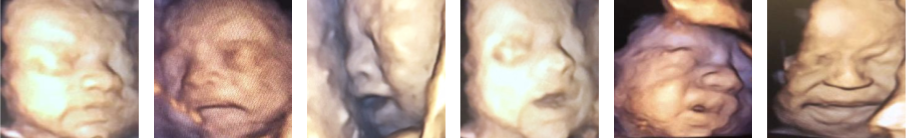
\includegraphics[height=2cm, keepaspectratio]{imgs/chap4_ap.png}
    \caption{Acute Pain Group}
  \end{subfigure}

  \par\bigskip

  \begin{subfigure}{\linewidth}
    \centering
    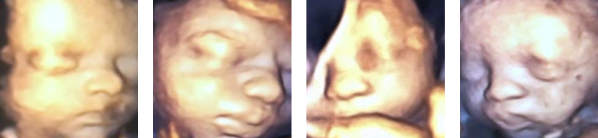
\includegraphics[height=2cm, keepaspectratio]{imgs/chap4_re.png}
    \caption{Rest Group}
  \end{subfigure}

  \par\bigskip

  \begin{subfigure}{\linewidth}
    \centering
    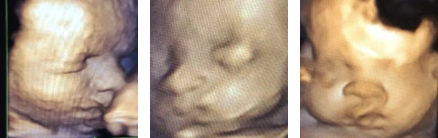
\includegraphics[height=2cm, keepaspectratio]{imgs/chap4_as.png}
    \caption{Acoustic Stimulus Group}
  \end{subfigure}
  
  \caption{Images of each individual fetus grouped by their conditions.}
  \label{fig:fetuses}
\end{figure}  
